\documentclass[12 pt]{article}
\usepackage{amsmath,amsfonts,parskip}
\usepackage[a4paper]{geometry}
\usepackage[T1]{fontenc}
\usepackage{enumerate}
\usepackage{graphicx}

\begin{document}

\begin{center}
       \large{
       \textbf{Computational Physics - PH3264} \break
	Module 2 - Integration
}
\end{center}

\textbf{Krishna Iyer V S \hfill Roll:20201017}
\hrule 
\vspace{0.3cm}

\begin{enumerate}[a.]

\item The function's actual integrand is $\pi$. The following plot shows the errors plotted against the number of bins on a log-log scale.
\begin{center}
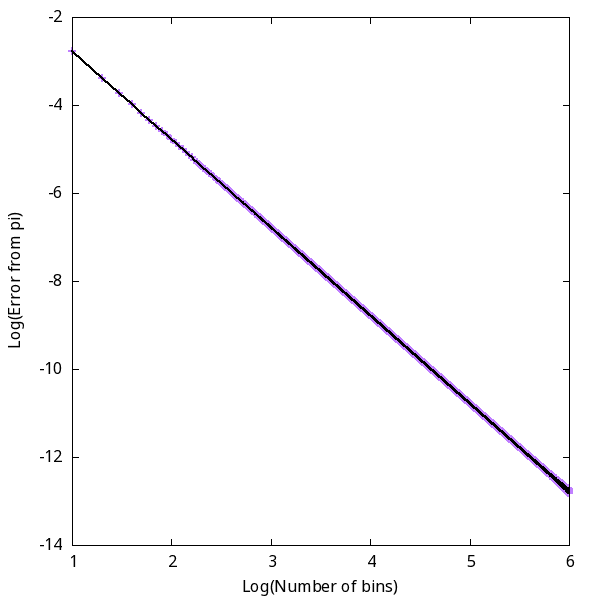
\includegraphics[width=3.5in]{"plots/log_log_q1_a.png"}
\end{center}
\end{enumerate}
\end{document}
